\documentclass[11pt]{article}

\newcommand{\Moser}{M{\"o}ser}

\usepackage{algorithm2e}
\usepackage[english]{babel}
\usepackage{cite}
\usepackage{float}
\usepackage[margin=1.5in]{geometry}
\usepackage{graphicx}
\usepackage{setspace}
\usepackage{tabularx}
\usepackage{url}

\bibliographystyle{acm}

\graphicspath{{figures}}

\onehalfspacing

\begin{document}
\begin{titlepage}
\title{Anonymity Analysis of Cryptocurrencies}
\author{Liam Morris \\
  \multicolumn{1}{p{.8\textwidth}}{\centering
  \begin{small}
  Department of Computer Science\\
  Rochester Institute of Technology\\
  Rochester, New York 14623 USA\\
  \end{small}
  {\tt lcm1115@rit.edu}\\\vspace{2em}
  \emph{Master's Thesis Proposal}\\\vspace{2em}
  Chair: Professor Stanis{\l}aw Radziszowski\hfill{\tt spr@cs.rit.edu}\\\vspace{1em}
  \hrulefill\\\vspace{1em}
  Reader: Professor Warren Carithers\hfill{\tt wrc@cs.rit.edu}\\\vspace{1em}
  \hrulefill}}
\date{March 3, 2013}
\end{titlepage}
\maketitle
\vfill
\begin{abstract}
A cryptocurrency is a form of electronic cash backed by mathematical and
cryptographical constructs, unlike traditional currency which was historically
backed by gold or silver. Cryptocurrencies have seen rising popularity in recent
years due to their decentralized, distributed, peer-to-peer protocols. Part of
this rising popularity is also attributable to the supposed anonymity of these
protocols. However, due to the public transaction history required for these
protocols, and the fact that transactions are psuedonymous and not purely
anonymous, this supposed anonymity may not exist. In this thesis we aim to
analyze the technical implementations of Bitcoin and other cryptocurrencies to
determine the level of anonymity provided by these protocols. We also aim to
research some improvements that have already been proposed to determine their
feasibility.
\end{abstract}
\thispagestyle{empty}
\clearpage
\pagenumbering{arabic}
\tableofcontents
\listoffigures
\pagebreak
\section{Problem Statement}
A cryptocurrency is a digital currency backed by mathematics and
cryptography, compared to traditional fiat money which was traditionally backed by gold
or silver. The foundation of many cryptocurrencies is based on a key derivation
scheme known as scrypt~\cite{percival09}.
Cryptocurrencies, such as Bitcoin~\cite{nakamoto08}, provide a means of having a
decentralized, distributed, peer-to-peer electronic cash system. These protocols
supposedly provide some level of anonymity, such that transactions and tender
cannot be directly associated with specific individuals. However, given the
technical specification of many cryptocurrencies, this anonymity may not exist
as stated.

\section{Cryptocurrency Protocols}
Cryptocurrency protocols generally consist of three main components: a
transaction scheme, a verification scheme, and a transaction ledger. The specific
details for each of these may vary between protocols, but they typically exhibit
the same characteristics regardless of specific implementation.

\subsection{Bitcoin Protocol}
Bitcoin is the most widely used cryptocurrency and is the first cryptocurrency
to begin circulation. Many other cryptocurrencies are direct forks of Bitcoin,
so the Bitcoin protocol will be our primary focus.

\subsubsection{Transaction Scheme}
The transaction scheme of Bitcoin uses psuedonyms to specify a transaction
between users on the network. A transaction is recorded as a transfer of some
value from one or more signatures to another signature.

\begin{minipage}{\linewidth}
The method of recording a new transaction of some bitcoin from User A to User
B is as follows:
\begin{enumerate}
    \item User A signs the bitcoin's previous transaction signature with User
        A's private key
    \item The resulting value is used as an input in a hash function along
        with User B's public key
    \item The output of this hash is the transaction signature, which can be
        signed with User B's private key to initiate another transaction
\end{enumerate}
\end{minipage}
\begin{figure}[H]
    \centering
    \caption[Bitcoin transaction process]{Bitcoin transaction process~\cite{nakamoto08}}
    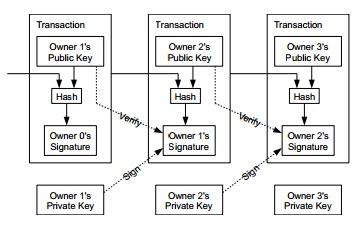
\includegraphics{figures/transaction.png}
\end{figure}

Once a transaction has been created, it is sent out to the Bitcoin network in
order to be verified.

\subsubsection{Verification Scheme}
Once a transaction has been initiated, it must be verified by users in the
Bitcoin network in order for the transaction to be fully committed. Verification
of a transaction requires some proof-of-work in order to complete the block and
append it to the block chain. The proof-of-work scheme used by the Bitcoin
protocol is based on the Hashcash proof-of-work scheme~\cite{back02}. 
To complete proof-of-work for some transaction, a
SHA-256 hash with inputs of the previous hash and some nonce must be found such
that the resulting hash is below some difficulty level. In other words, we must
feed the SHA-256 algorithm the previous hash of the coin concatenated with some
nonce such that we have a specified number of leading 0's in the resulting hash.
One common way of computing proof-of-work is using the following algorithm:
\begin{algorithm}[H]
    \KwIn{$D$ = difficulty parameter, $P$ = previous transaction hash}
    \KwOut{nonce, resulting hash}
    $N \gets 0$\\
    $H \gets ${\sc SHA-256($P + N$)}\\
    \While{H $\ge$ D}{
        $N \gets N + 1$\\
        $H \gets ${\sc SHA-256($P + N$)}
    }
    \Return{N, H}
\end{algorithm}\vspace{1em}

Once a proof-of-work has been determined, the block with the proof-of-work
information is distributed to the Bitcoin network. The difficulty of the
proof-of-work operation is such that blocks are found for a transaction, on
average, in 10 minutes.

\subsubsection{Network Structure}
The original Bitcoin whitepaper~\cite{nakamoto08} describes the Bitcoin network in the following
way:
\begin{enumerate}
    \item Transactions are broadcast to all network nodes.
    \item Transactions are collected and joined to form a block.
    \item A proof-of-work for a block is found which is broadcast to all nodes.
    \item If the proof-of-work is valid, all transactions in a block are valid,
        and transactions have not already been spent, then block is accepted.
    \item The accepted block is appended to the block chain, and its hash is now
        used as the input hash for the next block.
\end{enumerate}

In other words, all nodes in the network are made aware of new transactions,
verified transactions, and accepted blocks. In this way, the transaction record
(block chain) is shared among all nodes in the network.

\subsection{Litecoin Protocol}
Litecoin is one of the most widely used cryptocurrencies, and is itself a fork
of Bitcoin. The primary difference between Litecoin and Bitcoin is how the coins
are mined, or rather how the transactions are verified. Litecoin aims to have
transactions confirm faster with an average time of 2.5 minutes, as well as
reduce the benefit of special purpose hardware for mining coins~\cite{ahamad13}.
Although Litecoin is itself a fork of Bitcoin, many forks of Litecoin have been
created, so Litecoin is worth some analysis.

\subsubsection{Transaction Scheme}
The Litecoin transaction scheme is identical to that of
Bitcoin. Litecoin also records the signatures of all users involved, the amount
being transferred, etc.\ in a block, which is then itself part of a larger block
chain.

\subsubsection{Verification Scheme}
Litecoin was forked from Bitcoin to address the strength that special purpose
hardware brings to Bitcoin. Users in the Bitcoin network with application
specific integrated circuits (ASIC) design specifically for computing SHA-256
hashes have an enormous advantage over users without such hardware. To address
this, Litecoin uses the scrypt hashing scheme instead of SHA-256, which changes
the hashing scheme from a CPU-bound operation to a memory-bound operation. By
changing the verification problem from a CPU-hard to memory-hard problem,
parallelization no longer improves the speed of solving the
problem~\cite{percival09}. This yields the following Litecoin proof-of-work
algorithm:
\begin{algorithm}
    \KwIn{$D$ = difficulty parameter, $P$ = previous transaction hash}
    \KwOut{nonce, resulting hash}
    $N \gets 0$\\
    $H \gets ${\sc scrypt($P + N$)}\\
    \While{H $\ge$ D}{
        $N \gets N + 1$\\
        $H \gets ${\sc scrypt($P + N$)}
    }
    \Return{N, H}
\end{algorithm}

\subsubsection{Network Structure}
The network structure of Litecoin, much like the transaction scheme, is
virtually identical to that of Bitcoin. The network nodes are users connected to
the network, who receive notifications of new transactions and verified
transactions.

\subsection{Current State of Anonymity}
Users in the Bitcoin community can be falsely led to the conclusion that their
transactions are purely anonymous. For example, WikiLeaks accepts bitcoin
donations, stating that\footnote{\url{http://shop.wikileaks.org/donate} --
Accessed: 3-25-14},
\begin{quote}
``Bitcoin is a secure and anonymous digital currency. Bitcoins cannot be easily
tracked back to you, and are safer and faster alternative to other donation
methods.''
\end{quote}
This quote was published in 2011, yet still remains as stated on the WikiLeaks
website as of March 2014 despite some criticism of its accuracy.

Each transaction contains identifying information with respect to the addresses
of the users. For every transaction in the block chain, we can see between which
users the transaction occurred, as well as the number of bitcoins transferred.
Each of these transactions exists in the public transaction record to defend
against double spending of bitcoins. Due to the public nature of this record and
the information associated with each transaction, it is possible to deduce some
information about users on the network.

One way to deduce information about users is based on the input addresses into a
transaction. Since the private key owning a bitcoin is required to initiate a
transaction of that bitcoin, then we can safely assume that in a transaction
that contains multiple input addresses, that those addresses belong to one
entity or person. The other possible scenario is that private keys were shared,
but this is an unlikely scenario. In fact, in the original Bitcoin whitepaper,
Nakamoto states~\cite{nakamoto08},
\begin{quote}
``Some linking is still unavoidable with multi-input
transactions, which necessarily reveal that their inputs were owned by the same
owner.''
\end{quote}

Much research has been done in this area already. In 2011, Reid and Harrigan
analyzed one specific case of a theft of 25,000 BTC and attempted to trace the
stolen BTC through the Bitcoin network~\cite{reid11}. One of the important
results from this study was that it was not extraordinarily difficult to follow
the transfer of bitcoins between entities. The two were able to successfully
trace the stolen bitcoins across many transfers and determine some specific
addresses to which the coins were transferred, such as LulzSec.

One way in which Nakamoto addresses this is suggesting that public keys be kept
anonymous. However, this is not always ideal or even practical. Many users
publish their public keys in forum signatures so that they may receive bitcoins.
In this case, the public key is then very obviously associated with that
specific username, and passive analysis of multi-input transactions can possibly
reveal other keys associated with that user. Even if users do not publish their
keys in this way, some association may be revealed if a user takes advantage of
services or stores that accept bitcoins. Consider the case of a user wanting to
exchange her bitcoins for some form of currency. To do so, she must go through
some Bitcoin exchange service, in which she necessarily reveals some personally
identifying information to be able to receive her money. She has now placed her
anonymity in the hands of the exchange, since if the exchange is compromised,
her personal information is now compromised as well.

In 2013, Ron and Shamir~\cite{ron13} performed analysis on the Bitcoin network
using transaction size as their metric. First they performed similar analysis to
Reid and Harrigan to build a graph of entities, and then analyzed large
transactions to and from those entities. One of the first results from this
analysis is that the two were able to easily identify a few key entities: Mt.
Gox (the largest bitcoin exhange at the time, filed for bankruptcy February 28,
2014), Instawallet (another large bitcoin exhange, shut down April 3rd, 2013),
and DeepBit (the largest mining pool at the time).

Another key result determined
from this analysis is the transaction patterns that are commonly used to attempt
to obscure a user's identity. The main activities identified by Ron and Shamir
are long chains, fork-merge patterns, and savings accounts. The long chains of
transactions begin as one or more large transactions, which are then split into
many smaller transactions in a very long chain. Fork-merge patterns are similar,
except that the smaller transactions are eventually merged back into one
address. A large transaction gets split into multiple smaller transactions, but
all bitcoins ultimately end up back at the originating address. The last
activity observed was the use of Bitcoin "savings accounts." Bitcoins are
distributed across many addresses, after which they are essentially untouched. A
common pattern for all of these activities is splitting a transaction into equal
parts, which are then also split into equal parts, etc. The resulting structure
observed from this activity is akin to a binary tree.

Researchers at University of California, San Diego and George Mason
University~\cite{meiklejohn13} performed analysis on change addresses in a
Bitcoin transaction. Meiklejohn et al.\ used the assumption that a one-time
change address is controlled by the same user as the input addresses. Based on
this assumption, the group was able to discover what they called "peeling
chains," similar to activities observed by Ron and Shamir. This type of analysis
was applied to a rather peculiar Bitcoin wallet\footnote{\tt
1DkyBEKt5S2GDtv7aQw6rQepAvnsRyHoYM}, in which an extremely large Bitcoin wallet
was split into several smaller wallets. These smaller wallets then eventually
interacted with some Bitcoin services, including exchanges. If this wallet were
associated with an entity such as the Silk Road or the Bitcoin Savings \& Trust
Ponzi scheme~\cite{moore13}, the exchanges might be inclined to reveal
identifying information about the user in question, ultimately eliminating any
notion of anonymity.

Using the result from these studies, we can clearly see that input addresses and
change addresses can be used to identify Bitcoin "entities." We can also analyze
these entities more closely and see how the entities try to obscure their
identity. Since these sorts of patterns are not extraordinarily difficult to
deduce from the Bitcoin block chain, one can imagine a scenario where some law
enforcement agency might want to investigate a user who is a suspect in some
sort of illict activity. We can determine a group of addresses that belong to
the user, and if the user interacted with any sort of Bitcoin exchange or
service, the law enforcement agency could potentially seize the personal
information of the user form such a service. Even further, we can see all
addresses with which the user interacted, which could implicate other users
involved in illicit activities. This allows the law enforcement agency to
closely analyze these users more closely, some of which may have interacted with
a Bitcoin exchange, and so on.

\subsection{Improving Anonymity}
There have been many attempts to resolve the anonymity issues present in the
Bitcoin protocol. Some of these attempts have arisen organically within the
Bitcoin community and are already in use, while others are proposed by academic
papers and have yet to be implemented.

\subsubsection{Mixer}
A very common form of obscuring one's identity is to use a mixer or
tumbler\footnote{This name comes from the devices used to clean physical coins.}.
These services are based on mix networks~\cite{chaum81}, which are used to mask
a user's identity within a network, such as the commonly used Tor network.
However, unlike mix networks which are used to mix messages and anonymize the
users, Bitcoin mix services mix transactions to anonymize the users, frequently
charging some sort of processing fee for the service.

\begin{figure}[H]
    \caption[Example mix network]{Example mix network\protect\footnotemark}
    \centering
    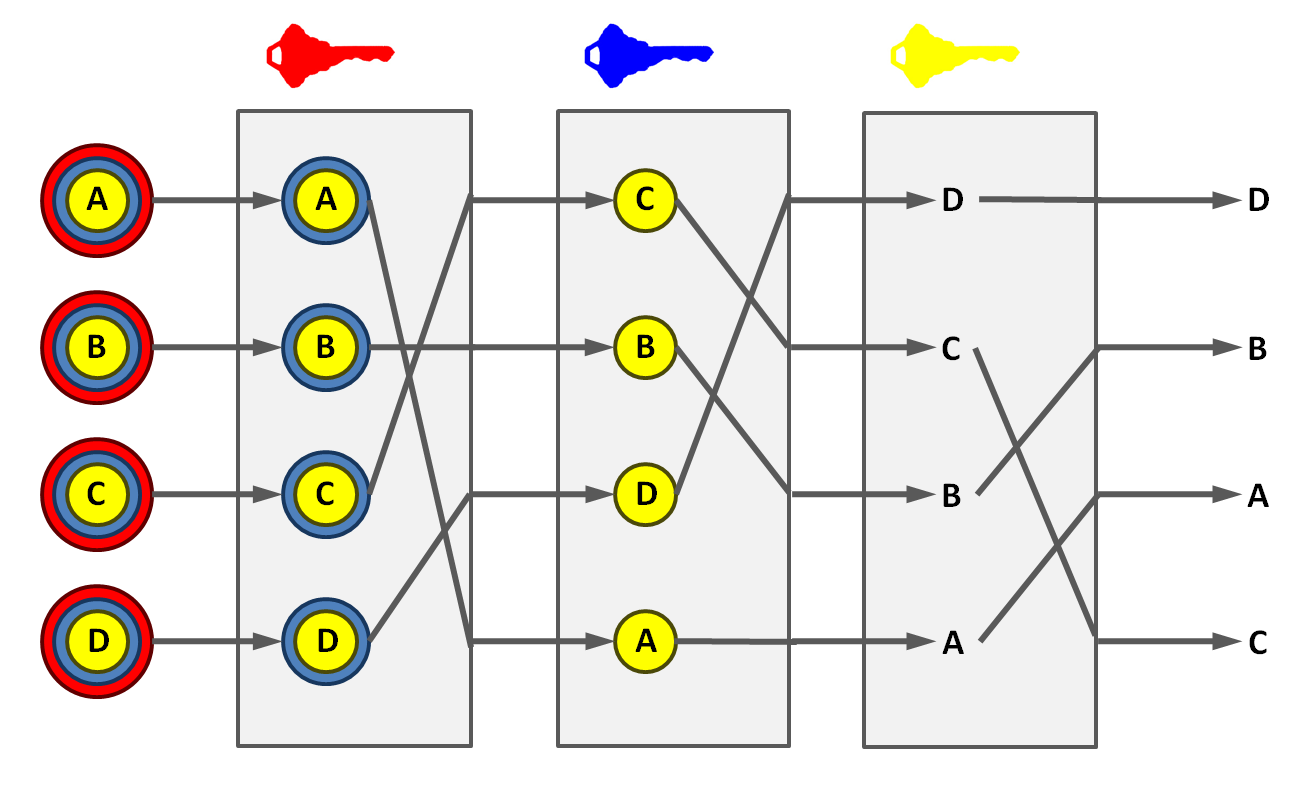
\includegraphics[width=.8\linewidth]{figures/mix.png}
\end{figure}

\footnotetext{\url{http://en.wikipedia.org/wiki/Mix_network} -- Accessed:
3-25-14}

Much work has been done to analyze the anonymity provided by these services.
In 2013, \Moser et al.\ analyzed three popular mixing services: Blockchain.info,
Bitcoin Fog, and BitLaundry~\cite{moser13}. The key results of this experiment
were that Blockchain.info and Bitcoin Fog both used complex methods of
distributed transactions that prevented the ability to discover any connection
between input and output transactions, effectively anonymizing the traffic.
BitLaundry, on the other hand, used direction connections between input and
output, which allows for connections to be drawn across the mixing operations.
This imperfect anonymization is present in other mixers, as in another study it
was observed that Bitcoin Laundry took input transactions and directly fed them
to output transactions, effectively eliminating the purpose of the
service~\cite{meiklejohn13}. The possible cause for this is that the pool of
users in the service is to small to sufficiently anonymize transactions.

One of the primary issues in using these mixing or laundry services is that
trust must be placed in the service, which is not an ideal scenario given that
one of the goals of Bitcoin is to eliminate the requirement to place trust in
individuals. It has even been observed that these services cannot necessarily be
trusted, as Meiklejohn et al.\ reported that ``One of these, BitMix, simply
stole our money.'' The presence of this behavior and the desire for anonymity
suggests that there is a desire for a system to provide anonymity without the
need to place trust in some sort of central figure.

\subsubsection{Zerocoin}
In 2013, researchers at Johns Hopkins University proposed an extension to
improve Bitcoin's anonymity known as Zerocoin~\cite{miers13}. The group claims
that Zerocoin ``uses standard cryptographic assumptions and does not introduce
new trusted parties or otherwise change the security model of Bitcoin.'' The
basic idea is to add newly minted coins to an accumulator, and then with the
assistance of zero-knowledge proofs spend the coins from the accumulator without
revealing a user's identity.

The Zerocoin protocol essentially creates a currency within Bitcoin. To mint
zerocoins, a user adds his bitcoins to the Zerocoin accumulator and receives
serial numbers in return, which correspond to the zerocoins that were "minted."
To later redeem the coins, the user must initiate a "Zerocoin Spend" transaction
and specify an output Bitcoin address. Upon verification of the bitcoins'
presence in the accumulator, done through a zero-knowledge proof, the
corresponding bitcoin value is sent to the specified output address.

\begin{figure}[H]
    \centering
    \caption[Bitcoin block chain (a) and Zerocoin block chain(b)]{Bitcoin block
        chain (a) and Zerocoin block chain (b)~\cite{miers13}}
    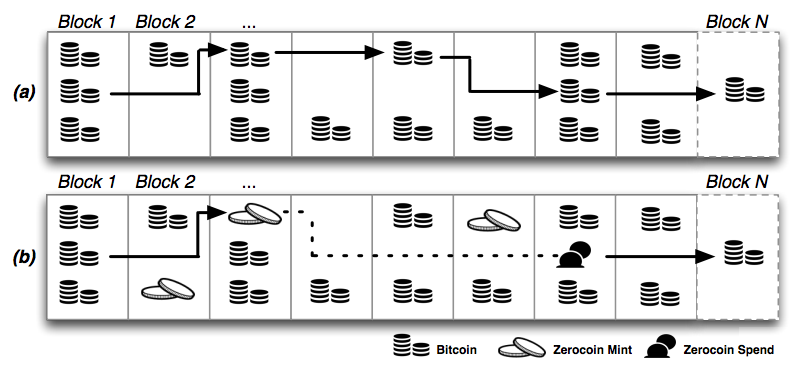
\includegraphics[width=\linewidth]{figures/zerocoin.png}
\end{figure}

This system creates anonymity by pooling all users' bitcoins together, and then
allowing for redemption of a random set of bitcoins from the pool, as long as
the user can prove that the bitcoins exist in the pool. In a sense, this is
analogous to a mixing service, but there is no requirement to place trust in any
figure, as the system is provably secure under certain cryptographic
assumptions.

\subsubsection{Mixcoin}
In 2014, another extension to improve anonymity in current Bitcoin protocol
was been proposed under the name of Mixcoin~\cite{bonneau14}. This protocol
describes a method of establishing mixing services with some concept of
warranty, rather than modifying the Bitcoin protocol itself.

In general, sufficiently large mixing services do an acceptable job at providing
anonymity to users. However, these services have an inherent risk in that users
must entrust the service with their bitcoins in order to utilize the service.
If a mixing service steals a user's bitcoins, there is no way to prove that the
theft occurred. Mixcoin's goal is to address this issue by proposing a
construction for a mixing service that has built-in accountability.

The basic process behind Mixcoin is that before any mixing occurs, a user Alice
contacts the mix service and declares the following
parameters~\cite{bonneau14}:\\
\begin{tabular}{cl}
    $v$ & the value (chunk size) to be mixed\\
    $t_1$ & the deadline by which Alice must send funds to the mix\\
    $t_2$ & the deadline by which the mix must return funds to Alice\\
    $\kappa_{out}$ & the address where Alice wishes to transfer her funds\\
    $\rho$ & the mixing fee rate Alice will pay\\
    $n$ & a nonce, used to pay randomized mixing fees\\
    $w$ & the number of blocks the mix requires to confirm Alice's payment
\end{tabular}\vspace{1em}\\
Once the mix accepts the terms of the mix, a new escrow address $\kappa_{esc}$
is generated. All parameters plus $\kappa_{esc}$ are returned to Alice, signed
by the mixing service. This allows Alice to publicly claim with certainty that
the mixing service has stolen her funds in the event of theft, or in the case
that the funds have not been delivered to $\kappa_{out}$ by $t_2$.

\section{Proposed Work}
The first part of research will consist of continued analysis of existing
research into cryptocurrency anonymity as well as existing proposals to address
cryptocurrency anonymity. It is clear that a great deal of attention has already
been directed towards the anonymity of the Bitcoin protocol, but similar
research and analysis has not been performed on other cryptocurrencies, such as
Litecoin.

We will investigate anonymity concerns of other cryptocurrency protocols and
determine if there are parallels with the Bitcoin community. If this is the
case, we will see what attempts (if any) have been made to address privacy
issues, as well as see if proposals to anonymize Bitcoin can be applied these
cryptocurrencies. Additionally, research that has been performed on the Bitcoin
transaction graph, such as identifying entities based on transaction inputs,
will be performed on the transaction graphs of other cryptocurrencies.

After researching current implementations and proposals it is important to
determine their feasibility. Indeed, one of the main goals of this thesis is to
analyze the computational overhead required to add anonymity to
cryptocurrencies. This may require implementing these protocols through software
if no software implementations already exist. Once we have an implementation of
these systems, we will conduct performance benchmarking to determine the
computational complexity present in the protocols.

The ideal outcome of this work is that one or more of these systems can be
implemented with minimal computational cost. However, in the case that the base
systems are not computationally feasible, we will perform more in-depth research
into possible improvements that can be made to specific algorithms to improve
performance while maintaining the same overall functionality. It is possible
that such changes could be significant enough to warrant a formal writeup of a
new protocol, but this would be an accidental side-effect and not one of our
primary goals.

\section{Deliverables}
Upon completion of all proposed work, a thesis report will be submitted.
Contained in this thesis will be all background research, experiment results,
and any other required documentation. Additionally, the following software will
be submitted:
\begin{itemize}
    \item Libraries for any cryptocurrency extensions that are implemented
    \item Library for performing benchmarks on cryptocurrency systems
\end{itemize}

\section{Timeline}
The writing of the thesis, software implementation, and research will all be
done in parallel. A proposed schedule is as follows:
\begin{center}
\begin{tabularx}{\textwidth}{l|l}
    Date & Task\\
    \hline
    April 25, 2014 & Complete thesis proposal submission\\
    May 16, 2014 & Perform block chain analysis on Litecoin\\
    May 2014 -- August 2014 & \emph{Summer Co-op}\footnote{Research will
                              continue, but there is no formal timeline for
                              this period of time}\\
    September 5, 2014 & Finish required background research, begin software
                        implementation\\
    September 19, 2014 & Finish software implementation, begin benchmarking and
                         recording data\\
    October 3, 2014 & Complete data analysis, revisit software implementation
                      for optimizations\\
    October 17, 2014 & Benchmark optimizations and record changes\\
    November 14, 2014 & Finish Thesis Report\\
    December 12, 2014 & Defend Thesis\\
\end{tabularx}
\end{center}

\bibliography{references}

\end{document}
